% ===========================================================================
% SECTION 2 — SYSTEM MODELING
% Target: 600-800 words
% ===========================================================================

\section{System Modeling}
\label{sec:system_modeling}

\subsection{NREL 5-MW Reference Turbine}
\label{subsec:nrel5mw}

This study uses the NREL offshore 5-MW reference wind turbine
\cite{jonkman2009} as the physical plant. This model is widely adopted as a
benchmark in the wind energy control literature, which allows direct
comparison with previously published MPC and ML-surrogate studies. {\color{auditP2}The
turbine has a rotor radius $R = \SI{63}{m}$, a $97{:}1$ gearbox ratio, a rated rotor speed
$\omegarated = \SI{12.1}{rpm}$, and a rated generator torque (high-speed
shaft, HSS) $T_{g,\text{rated}} = (P_{\text{rated}}/\eta_{\text{gen}}) /
(\omegarated N_{\text{gear}}) = \SI{43093.55}{N.m}$, using the
reference generator efficiency $\eta_{\text{gen}}=94.4\%$
\cite{jonkman2009}, so that rated electrical power
$P_{\text{rated}}=\SI{5}{MW}$ corresponds to $\SI{5.2966}{MW}$ of
rated mechanical power on the low-speed shaft. The inertia used in the
two-state model, $J = 3.876 \times 10^{7}~\text{kg}\cdot\text{m}^2$
(referred to the low-speed shaft, LSS), is the rotor inertia obtained from
the blade and hub properties of~\cite{jonkman2009}; the generator inertia
($N_{\text{gear}}^{2} I_{\text{gen}} \approx 5.03\times10^{6}~\text{kg}\cdot\text{m}^2$)
is neglected, so that $J$ underestimates the full drivetrain inertia by
about $11.5\%$.} An earlier draft of
this paper omitted this efficiency division, giving
$\SI{40680}{N.m}$ ($5.6\%$ low); this has been corrected to adopt the
reference value directly, propagated through the Region~II gain
$\Kopt$ below and the torque-switching law of
Section~\ref{subsec:torque_switching}. The rated tip-speed ratio is
$\lambda_{\text{rated}} = 7.00$. Full turbine parameters are reported in
Table~\ref{tab:turbine_params}.

\begin{table}[H]
\centering
\caption{{\color{auditP2}Turbine parameters of the two-state model used in this study.
Rotor radius, number of blades, air density, gear ratio, maximum pitch rate,
rated rotor speed, rated power, rated, cut-in and cut-out wind speeds and
rated generator torque are those of the NREL 5-MW reference turbine
(Jonkman \emph{et al.}~\cite{jonkman2009}); $\lambda_{\text{rated}}$ is
computed from the reference $R$, $\omegarated$ and $V_{\text{rated}}$, and
$\Kopt$ is the reference generator-side Region~2 gain
(\SI{0.0255764}{N.m/rpm^2}) referred to the low-speed shaft. $J$ is the rotor
inertia obtained from the reference blade and hub properties (generator
inertia neglected). The viscous rotor damping $B_r$, pitch actuator time
constant $\tau_\beta$, pitch bounds, minimum rotor speed and overspeed limit
are modeling choices of this study and are not taken from~\cite{jonkman2009},
which specifies pitch settings of $0\deg$ to $90\deg$, a minimum rotor speed
of \SI{6.9}{rpm} and a drive-shaft torsional damping rather than a viscous
rotor damping.}}
\label{tab:turbine_params}
\begin{tabular}{lcc}
\toprule
Parameter & Symbol & Value \\
\midrule
Rotor radius              & $R$                 & \SI{63}{m} \\
Number of blades          & $B$                 & 3 \\
Air density                & $\rho$              & \SI{1.225}{kg/m^3} \\
{\color{auditP2}Rotor inertia (LSS)}        & {\color{auditP2}$J$}                 & $3.876\times10^{7}$ kg$\cdot$m$^2$ \\
{\color{auditP2}Viscous rotor damping}      & {\color{auditP2}$B_r$}               & \SI{6215.5}{N.m.s/rad} \\
Gear ratio                 & $N_{\text{gear}}$   & 97 \\
Pitch actuator time constant & $\tau_\beta$      & \SI{0.1}{s} \\
Pitch bounds                & $\beta$             & $[0,\ 25]\deg$ \\
Maximum pitch rate          & $\dot\beta_{\max}$  & \SI{8.0}{deg/s} \\
Rated rotor speed          & $\omegarated$       & \SI{12.1}{rpm} \\
{\color{auditP2}Min.\ rotor speed (numerical guard)} & {\color{auditP2}$\omega_{\min}$}     & \SI{4.77}{rpm} \\
Overspeed limit (+10\%)    & $\omega_{\max}$     & \SI{13.31}{rpm} \\
Rated tip-speed ratio       & $\lambda_{\text{rated}}$ & 7.00 \\
Rated power                & $P_{\text{rated}}$  & \SI{5}{MW} \\
Rated wind speed           & $V_{\text{rated}}$  & \SI{11.4}{m/s} \\
Cut-in wind speed          & $V_{\text{in}}$     & \SI{3.0}{m/s} \\
Cut-out wind speed         & $V_{\text{out}}$    & \SI{25.0}{m/s} \\
Rated generator torque (HSS) & $T_{g,\text{rated}}$ & \SI{43093.55}{N.m} \\
Region II gain (LSS)        & $\Kopt$             & $2.128616\times10^{6}$~N.m.s$^2$ \\
\bottomrule
\end{tabular}
\end{table}

\subsection{Two-State Model}
\label{subsec:two_state_model}

{\color{auditP2}The turbine is
represented by a reduced two-state nonlinear model with state vector
$x = [\omegar, \beta]^\top$, control input $u = \betacmd$ (pitch angle
demand), and measured disturbance $V$ (rotor-effective wind speed). By
comparison, the control-oriented model of Klein \emph{et al.}~\cite{klein2024}
has eight states, among which the rotor speed and the mean pitch angle, two
inputs (pitch and generator-torque demands), and treats the rotor-effective
wind speed as an estimated disturbance state rather than a measurement.} The
rotor dynamics are governed by the aerodynamic torque balance

\begin{equation}
J\,\dot{\omegar} = \Ta(\omegar, \beta, V) - \Tg^{\text{LSS}}(\omegar) - B_r\,\omegar,
\label{eq:rotor_ode}
\end{equation}

where $\Tg^{\text{LSS}}$ is the generator reaction torque referred to the
low-speed shaft (Section~\ref{subsec:torque_switching}), $B_r =
\SI{6215.5}{N.m.s/rad}$ is a linear drivetrain damping coefficient
(Table~\ref{tab:turbine_params}), and the
aerodynamic torque is
$\Ta = \tfrac{1}{2}\rho \pi R^2 V^3 \Cp(\lambda,\beta) / \omegar$, with tip-speed
ratio $\lambda = \omegar R / V$ and {\color{auditP2}power coefficient surface
$\Cp(\lambda,\beta)$ evaluated with the six-coefficient empirical approximation
given below.} The pitch
actuator is modeled as a first-order lag,

\begin{equation}
\tau_\beta\,\dot{\beta} = \betacmd - \beta,
\label{eq:pitch_actuator}
\end{equation}

with $\tau_\beta = \SI{0.1}{s}$. Equations~\eqref{eq:rotor_ode}--\eqref{eq:pitch_actuator}
are integrated with explicit Euler discretization at $\Delta t = \SI{0.1}{s}$,
matching the control sampling time $T_s$ used by the nonlinear MPC in
Section~\ref{sec:mpc_framework}. The $\Cp(\lambda,\beta)$ surface is
{\color{auditP2}evaluated within the domain $\beta \in [0\deg, 25\deg]$,
$\lambda \in [2, 13]$ adopted in this study; this paper uses a widely used
six-coefficient empirical approximation of the $C_p(\lambda,\beta)$ surface,
$C_p = c_1(c_2/\lambda_i - c_3\beta - c_4)e^{-c_5/\lambda_i} + c_6\lambda$,
with $1/\lambda_i = 1/(\lambda + 0.08\beta) - 0.035/(\beta^{3}+1)$ and
$c_1, \ldots, c_6 = 0.5176, 116, 0.4, 5, 21, 0.0068$, clipped to
$[0,\,16/27]$.}

Stage=0 validation confirmed a maximum power coefficient $C_{p,\max} = 0.480$ at $\lambda^* = 8.11$, $\beta^* = 0^\circ$, safely below the Betz limit ($C_{p,\text{Betz}} = 0.5926$), correcting an earlier non-physical evaluation of the polynomial outside its calibrated range that had produced $C_{p,\max} = 0.706 > C_{p,\text{Betz}}$. This peak value agrees closely with the reference-reported peak of $0.482$ \cite{jonkman2009} (within $0.4\%$), but at a different tip-speed
ratio: the reference reports its peak at $\lambda=7.55$, whereas this
exact polynomial, evaluated numerically over a fine grid, peaks at
$\lambda=8.10$--$8.11$. {\color{auditP2}This displacement matters beyond Section~2.2 itself:
the Region~II gain used in this paper is the reference gain, derived at the
reference peak ($\lambda=7.55$), and is therefore not tuned to the peak of
this paper's own $\Cp$ surface (Section~\ref{subsec:torque_switching}).}

\subsection{Region II/III Generator Torque Switching}
\label{subsec:torque_switching}

A methodological contribution of this work concerns the generator torque
model $\Tg^{\text{LSS}}(\omegar)$ in Eq.~\eqref{eq:rotor_ode}. An initial
implementation assumed a constant rated torque
$\Tg^{\text{LSS}} = N_{\text{gear}}\,T_{g,\text{rated}}$ at all rotor
speeds. Under this assumption, long-horizon closed-loop simulation revealed
an irrecoverable operating trap: for $\omegar$ below the rated speed, the
aerodynamic torque $\Ta$ available at low wind speed can fall below the
constant demanded generator reaction torque, driving $\dot{\omegar} < 0$
with no control authority left to arrest the deceleration (the pitch angle
is already saturated at its lower bound $\beta = 0\deg$), so the rotor
stalls toward zero speed.

This was corrected by replacing the constant-torque assumption with the
standard Region~II/III generator torque switching law, expressed
consistently in low-speed-shaft (LSS) torque on both sides,

\begin{equation}
\Tg^{\text{LSS}}(\omegar) =
\begin{cases}
\Kopt\,\omegar^{2}, & \omegar < \omegarated \quad \text{(Region II)} \\[4pt]
N_{\text{gear}}\,T_{g,\text{rated}}, & \omegar \geq \omegarated \quad \text{(Region III)}
\end{cases}
\label{eq:torque_switching}
\end{equation}

where $\Kopt = \tfrac{1}{2}\rho A_{\text{rotor}} \Cp(\lambda_{\text{rated}})
R^3 / \lambda_{\text{rated}}^3 \approx 2.51\times10^{6}~\text{N.m.s}^2$ using
this paper's own $\Cp(\lambda,\beta)$ surface (Section~\ref{subsec:two_state_model});
the value actually used throughout this paper
(Table~\ref{tab:turbine_params}), $\Kopt=2.128616\times10^{6}~\text{N.m.s}^2$,
{\color{auditP2}instead adopts the generator-side Region~2 gain published by
Jonkman \emph{et al.}~\cite{jonkman2009},
$K_{\text{gen}}=\SI{0.0255764}{N.m/rpm^2}$, referred to the low-speed
shaft ($\Kopt=K_{\text{gen}}N_{\text{gear}}^3$, with the appropriate
rpm-to-rad/s unit conversion), $15.2\%$ lower than this paper's own
aerodynamic-formula estimate.\\ 
\textbf{Origin of the deviation}:
the two values are not calibrated at the same operating point.
Jonkman \emph{et al.}~\cite{jonkman2009} derive $K_{\text{gen}}$ from the
peak power coefficient of the reference rotor ($0.482$ at a tip-speed
ratio of $7.55$ and $0\deg$ pitch) and the $97{:}1$ gearbox ratio, whereas
the estimate above evaluates this paper's own $\Cp(\lambda,\beta)$ surface
at $\lambda_{\text{rated}}=7.00$.} {\color{auditP2}The
reference value is used throughout this paper because it does not
depend on this paper's own approximate $\Cp$ surface. The aerodynamic-formula
estimate above is evaluated at the rated operating point
$\lambda_{\text{rated}} = R\,\omegarated / V_{\text{rated}} = 7.00$, computed
from the reference values of~\cite{jonkman2009}, rather than at the
theoretical aerodynamic optimum $\lambda^{*} = 8.11$ of
Section~\ref{subsec:two_state_model}; it is given for comparison only, since
$\Kopt$ itself is not recalibrated in this study.} The
resulting continuity ratio, computed using the corrected
$T_{g,\text{rated}}=\SI{43093.55}{N.m}$ (HSS, item 3.1) and
$\Kopt=2.128616\times10^6$ (item 3.2) together -- an earlier draft
inconsistently combined one corrected and one uncorrected value here
-- is
$\Kopt \omegarated^{2} / (N_{\text{gear}} T_{g,\text{rated}}) = 0.8176$,
i.e.\ an $18.24\%$ torque shortfall at $\omegar = \omegarated$, stated
explicitly per shaft: on the low-speed shaft (LSS), Region~II torque
$\Kopt\omegarated^2 = \SI{3417632}{N.m}$ falls short of Region~III
torque $N_{\text{gear}}T_{g,\text{rated}} = \SI{4180075}{N.m}$ by
\SI{762442}{N.m}; equivalently, on the high-speed shaft (HSS),
$\Kopt\omegarated^2/N_{\text{gear}} = \SI{35233}{N.m}$ falls short of
$T_{g,\text{rated}}=\SI{43093.55}{N.m}$ by \SI{7861}{N.m}, the same
$18.24\%$ ratio (shaft-referral does not change the percentage, only
the absolute torque values). This is an order of magnitude larger
than an earlier draft's (internally inconsistent) figure, and we do
not dismiss it as automatically negligible on that basis alone;
instead, the same structural argument as before still applies and is
stated more carefully here: the explicit-Euler integration together
with continuous turbulent-wind excursions means the simulated system
has zero measure-theoretic probability of dwelling exactly at
$\omegar = \omegarated$, so a discontinuity confined to that single
point -- regardless of its magnitude -- does not by itself alter any
simulated trajectory; Section~\ref{sec:closed_loop_results}'s
closed-loop results, none of which show artifacts localized at
$\omegar=\omegarated$ specifically, are consistent with this. Feasibility of
Eq.~\eqref{eq:torque_switching} was validated by confirming
$\Ta(\omegar,\beta,V) - \Tg^{\text{LSS}}(\omegar) > 0$ for all
$\omegar \in [\omega_{\min}, \omegarated]$ and all $V$ in the operating
envelope, eliminating the trap. Fig.~\ref{fig:torque_switching} illustrates
$\Ta$ and $\Tg^{\text{LSS}}(\omegar)$ before and after the correction. This
correction also constrains the admissible rotor-speed range used for
surrogate-based MPC bounds in Stage~3
(Section~\ref{sec:mpc_framework}): the training domain identified in
Stage~1 (Section~\ref{sec:dataset_generation}) is $[8.02,13.31]$~rpm,
yielding surrogate MPC bounds of $[8.52,12.81]$~rpm with a
$\SI{0.5}{rpm}$ safety margin on each side, distinct from the wider
$[11.5,13.31]$~rpm defense-in-depth bound retained for the physics-based
Baseline controller.

\begin{figure}[H]
\centering
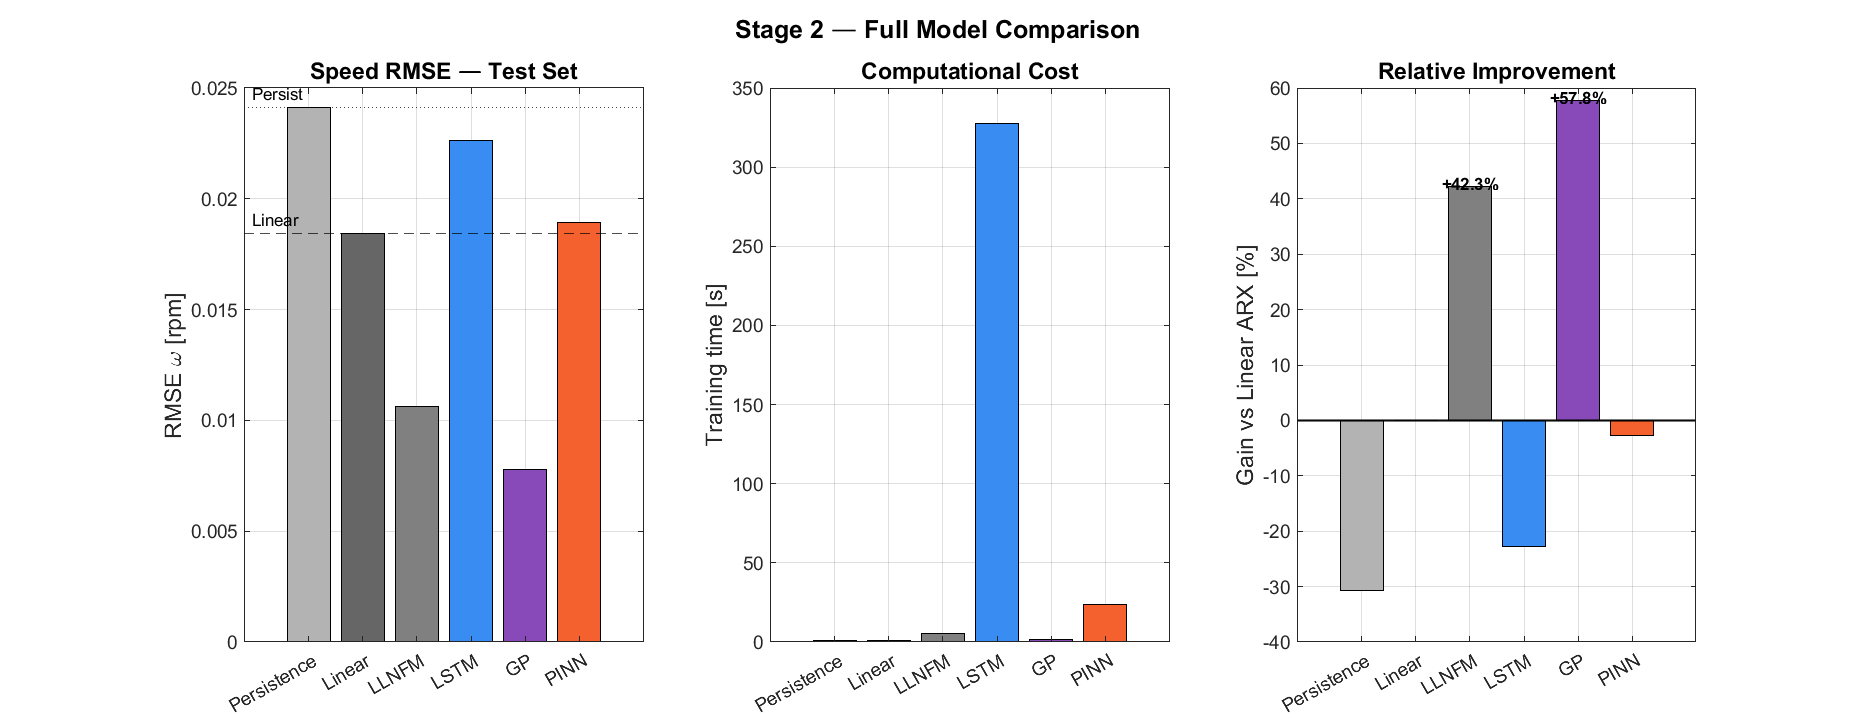
\includegraphics[width=0.8\textwidth]{figures/Fig3_S2_ModelSummary.png}
\caption{Region II/III generator torque switching: aerodynamic torque
$\Ta$ and generator torque $\Tg(\omegar)$ before (constant torque) and
after (Eq.~\eqref{eq:torque_switching}) correction.}
\label{fig:torque_switching}
\end{figure}

\subsection{Wind Model}
\label{subsec:wind_model}

{\color{auditP2}Turbulent wind input is generated from the Kaimal spectral model given in
the informative Annex~B of IEC~61400-1 \cite{iec61400}, with a constant
turbulence intensity $I = 0.16$, equal to the reference value
$I_{\text{ref}}$ of turbulence category~A, and longitudinal turbulence length
scale $L_1 = \SI{340.2}{m}$ ($L_1 = 8.1\,\Lambda_1$ with $\Lambda_1 = \SI{42}{m}$
for hub heights of \SI{60}{m} and above).} {\color{auditP2}We note that
$I=0.16$ is the reference turbulence intensity of IEC turbulence
category~A (categories A, B and C have $I_{\text{ref}} = 0.16$, $0.14$ and
$0.12$) rather than category~B ($I=0.14$) as an earlier draft of this work
mislabeled it; the simulated turbulence is therefore somewhat more severe
than a Category-B label would imply, not less.} Time series are
synthesized via inverse FFT of the discretized Kaimal power spectral
density, with the amplitude spectrum deterministically rescaled before
phase randomization so that the achieved standard deviation
$\sigma_{\text{actual}}$ matches the target
$\sigma_{\text{target}} = I \cdot V_{\text{mean}}$ \emph{by construction}
 this rescaling step is a normalization procedure, not an
independent validation of the synthesized turbulence, and should not
be read as evidence that the resulting time series matches the target
Kaimal spectrum in any property other than its overall standard
deviation. The achieved power spectral density is instead validated
independently against the analytical Kaimal spectrum in
Figure~\ref{fig:kaimal_psd}, using a periodogram
($\text{nfft}=N$, matching the theoretical spectrum's own frequency
resolution and avoiding the low-frequency-energy underestimation
that shorter-window methods such as Welch's method introduce).

\begin{figure}[H]
\centering
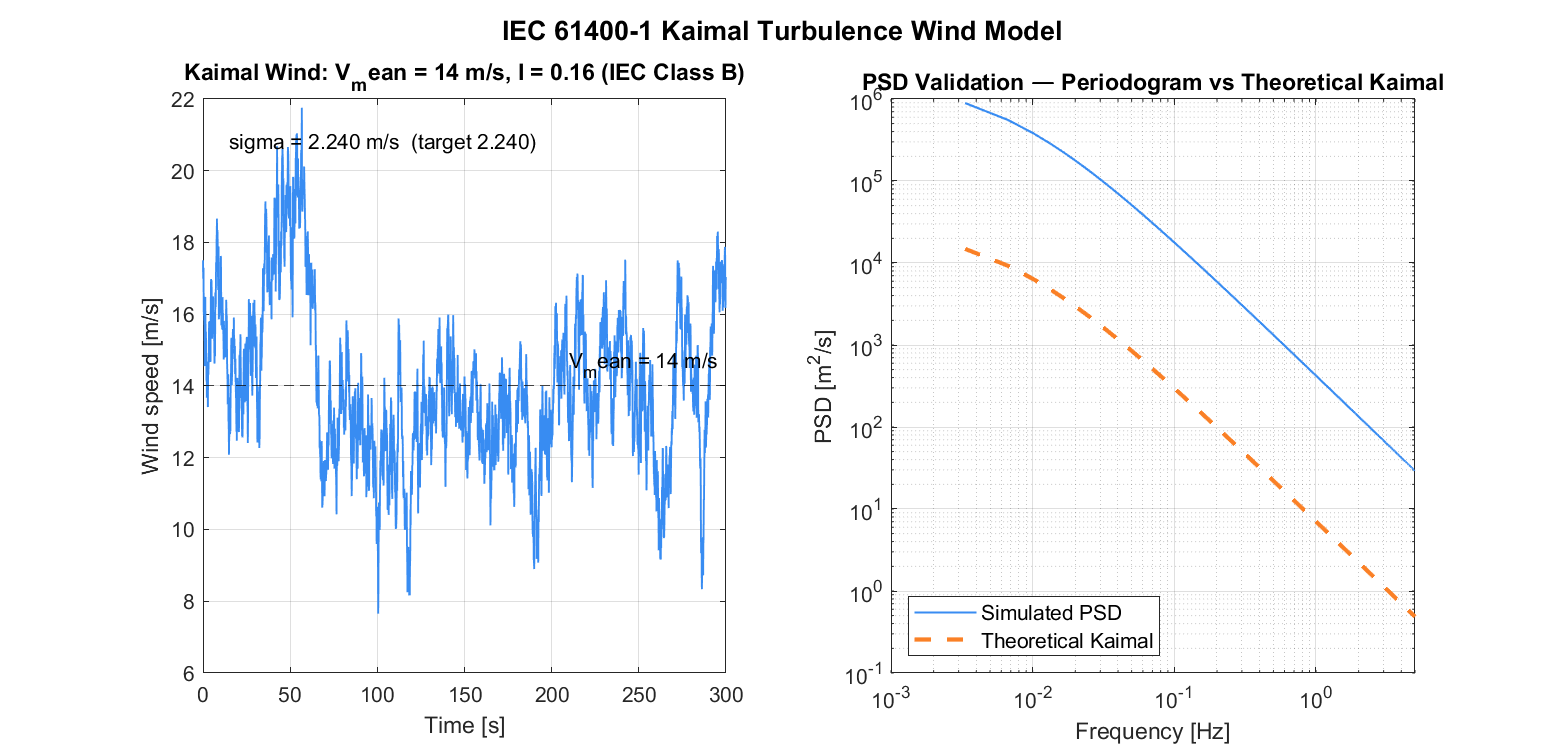
\includegraphics[width=0.85\textwidth]{figures/Fig0_4_Kaimal_PSD.png}
\caption{Achieved power spectral density (periodogram,
$\text{nfft}=N$) of a $T=\SI{300}{s}$ synthesized wind realization
($V_{\text{mean}}=\SI{14}{m/s}$, $I=0.16$) against the theoretical
Kaimal spectrum. This is an independent shape validation, distinct
from the by-construction standard-deviation match discussed in the
main text.}
\label{fig:kaimal_psd}
\end{figure}

{\color{auditP2}The
synthesized wind signal is subsequently passed through a second-order
Butterworth low-pass filter with cutoff frequency $f_c = \SI{0.3}{Hz}$
before being applied as the disturbance input $V$ to
Eq.~\eqref{eq:rotor_ode}.}
